\documentclass{scrartcl}
\usepackage{tikz}
\usetikzlibrary{arrows,automata}

\begin{document}
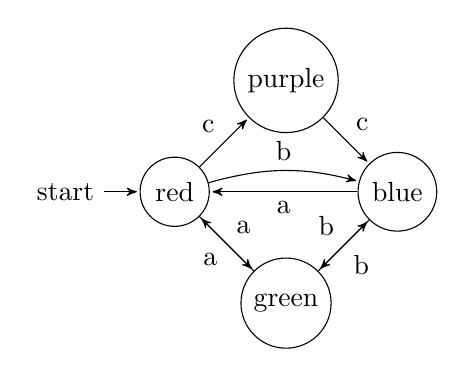
\begin{tikzpicture}[>=stealth',shorten >=1pt,auto,node distance=2cm]
  \node[initial, state]         (red)  {red};
  \node[state]         (green) [below right of=red] {green};
  \node[state]         (blue) [above right of=green] {blue};
  \node[state]         (purple) [above right of=red] {purple};


  \path[->]
  (red) edge node {a} (green)
  (red) edge [bend left = 15] node {b} (blue)
  (red) edge node {c} (purple)
  (green) edge node {a} (red)
  (green) edge node {b} (blue)
  (blue) edge node {a} (red)
  (blue) edge node {b} (green)
  (purple) edge node {c} (blue)
  ;
\end{tikzpicture}
\end{document}
